\documentclass[10pt]{beamer}
\usetheme{PaloAlto}
\usecolortheme{seahorse}
\setbeamertemplate{navigation symbols}{}
\setbeamertemplate{caption}[numbered]
%general package
%\usepackage[utf8]{inputenc}
\usepackage{array}
\usepackage[english]{babel}
\usepackage{geometry}
\usepackage{tcolorbox}
\usepackage[export]{adjustbox}
\usepackage{graphicx}
\usepackage{xcolor}
\graphicspath{{../img}}
\hypersetup{
    colorlinks=true, 
    linkcolor=red,    % Internal links
    urlcolor=blue     % External links
}
\usepackage{wrapfig}

%math package
\usepackage{amsmath}
\usepackage{amsfonts}
%\usepackage{amssymb}
%\usepackage{amsthm}
%\usepackage{slashed}
%\usepackage{tikz-cd}

%font package
%\usepackage{mathrsfs}
%\usepackage{bm}

%misc. package
\usepackage{enumitem}
\usepackage{animate}

\DeclareMathOperator{\xd}{\,d\!}
\DeclareMathOperator{\curl}{curl}
\DeclareMathOperator{\dive}{div}
\newcommand{\e}{{\rm e}}
\newcommand{\norm}[1]{\lVert#1\rVert}
\newcommand{\R}{\mathbb R}
\newcommand{\vF}{\mathbf F}
\newcommand{\vv}{\mathbf v}
\newcommand{\inpr}[1]{\left\langle#1\right\rangle}

\author[B.H.]{{\Large High School Geometry}\\\vspace{.5em} Instructor: Ben Huang}
\date{}
\title[Tangent]{The Tangent Ratio}

%\institute[MU]{\vskip -2em
\includegraphics[width = 0.65\textwidth]{CityPoly.png}}
%\logo{
\includegraphics[width=.12\textwidth]{CityPolySmall.png}}

\begin{document}
\frame{\titlepage}

\begin{frame}

{\bf Prerequisite Tools:} ruler, compass, and protractor
{
\begin{center}
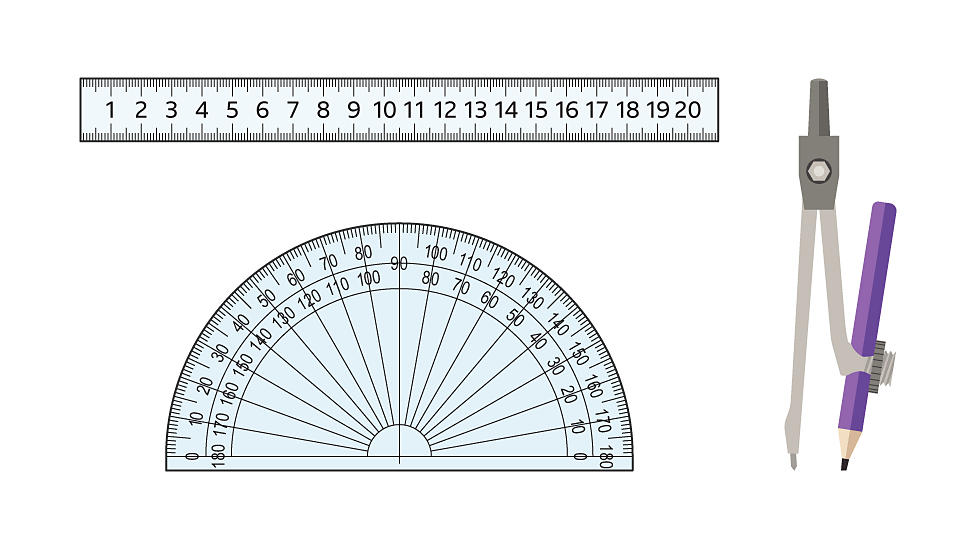
\includegraphics[width=0.75\textwidth]{geo-tools.png}
\end{center}
}
\end{frame}

\begin{frame}
\begin{wrapfigure}{r}{0.2\textwidth}
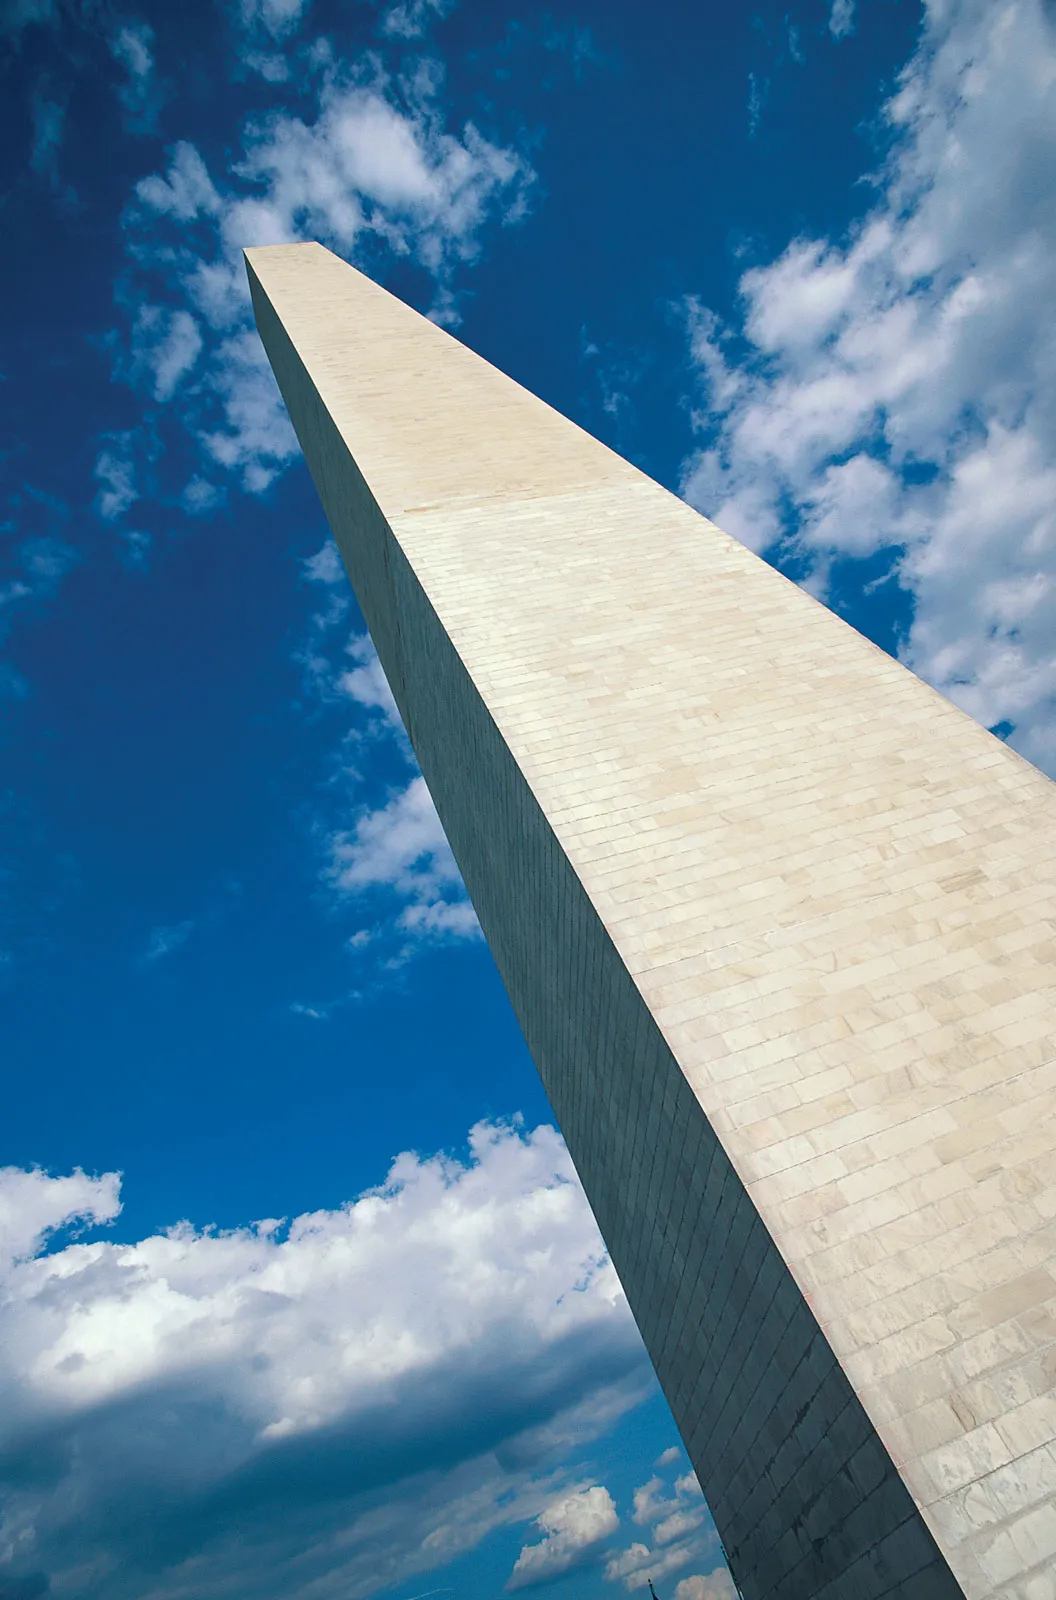
\includegraphics[width=1\linewidth]{washington-monument.png} 
\end{wrapfigure}
{\bf Question:} How tall is the Washington Monument?
\pause

{\bf According to \href{https://en.wikipedia.org/wiki/Washington_Monument}{Wikipedia}}: 555 ft
\pause

\vspace{\stretch{1}}

\begin{wrapfigure}{l}{0.2\textwidth}

\includegraphics[width=1\linewidth]{wondering.jpg} 
\end{wrapfigure}
Wait a minute...

\pause
How do we know this data is reliable?
\end{frame}

\begin{frame}
\begin{wrapfigure}{r}{0.3\textwidth}
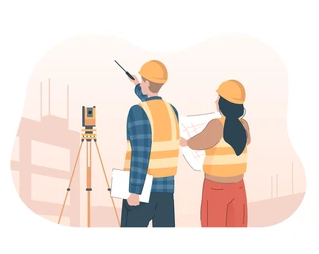
\includegraphics[width=1\linewidth]{surveyor.png} 
\end{wrapfigure}

If we want to measure the height on our own, how difficult would it be?\\
\pause
\vspace{\stretch{1}}

{\bf Hard to measure:} vertical distance\\
{\bf Easy to measure:} horizontal distance, angle of elevation
\pause

\href{https://youtu.be/yVF0Yeptn2c?si=Zz1jWbsK4En4H8nA}{Video: A simple device to measure the angle of elevation}
\end{frame}

\begin{frame}

{\bf The Mathematical Tool}: The Tangent Ratio
\pause
\begin{center}
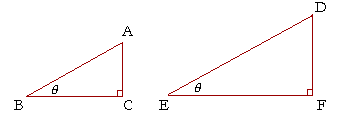
\includegraphics[width=0.8\textwidth]{similar-right-triangles.png}
\end{center}
\pause
\begin{align*}
\onslide<3->{\triangle ABC &\sim \triangle DEF \text{ (by the AA condition)}}\\
\onslide<4->{\frac{CA}{CB} &= \frac{FD}{FE}}
\end{align*}
\onslide<5->{
{\bf Definition:} In a right triangle,
\[
\tan(\theta) = \frac{\text{opposite side (opp)}}{\text{adjacent side (adj)}}
\]
}
\end{frame}

\begin{frame}

{\bf Problem:} A surveyor is standing 118 feet from the base of the Washington Monument. The surveyor measures the angle of elevation from the ground to the top of the monument to be $78^\circ$. Find the height $h$ of the Washington Monument to the nearest foot.
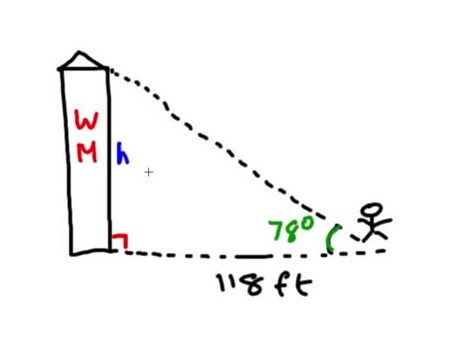
\includegraphics[width=0.4\textwidth, center]{washington-monument-surveyor.jpg}
\pause
\[
\tan(78^\circ) = \pause \frac{h}{118}
\]
\pause
\[
h=\pause118\tan(78^\circ)
\]
\end{frame}

\begin{frame}
To wrap up, let's find the approximate value of $\tan(78^\circ)$ together!

\href{https://www.geogebra.org/geometry}{GeoGebra}
\pause
\vspace{2em}

{\bf What's beyond:} In calculus, you will learn a method to find the value of tangent that is measure-error free via {\it infinite series}. 
\end{frame}

\end{document}